\subsection{Variational Quantum Algorithms}\label{Sec: Variational Quantum Algorithms}

Hybrid techniques involving quantum circuits and classical optimisers have been proposed to overcome the restrictions of Noisy Intermediate-Scale Quantum (NISQ) \cite{brooksQuantumSupremacyHunt2019} devices.
Those restrictions include inability of NISQ devices to achieve fault-tolerance, restrictions on the number of the available qubits per their quantum processors, and the limited depth of practically executable quantum circuits.
Moreover, quantum circuits and their gates are static by design, which means that input data into a quantum algorithm must be encoded as gates of the circuit implementing this algorithm. This implies that each instance of quantum algorithm use results in a new and distinct quantum circuit. This creates a barrier to using quantum circuits in support of efficient algorithm optimisation and training of quantum machine learning models.

Nevertheless, hybrid techniques, which combine classical and quantum techniques, allow development of \emph{variational circuits} (or circuit templates) with trainable parameters that can be iteratively refined by instantiating their values to create a static circuit using a traditional (classical) computer (i.e. when training VQAs) \cite{cerezo2021variational}, but which can then be efficiently executed on a quantum machine.
In this way, it is also possible to rely on range of classical optimisers, which treat variational circuits as black boxes capable of yielding outputs from inputs and the trainable parameters.

Consider a simple problem that we want to solve using VQA, given access to the training data.
The first step is to construct a \textit{cost function} $C$ used to search for an optimal set of circuit parameters, which is achieved by minimising the cost function during the training process.
We can simplify the development of variational circuits by composing the circuit templates called \textit{ansatze}.
\textit{Ansatz} is the parameterised circuit that depends on a set of parameters $\theta$. We aim to train the ansatze by optimising the parameters $\theta$s so that the cost function $C$ reaches its minimum, thus satisfying:
\begin{equation}
    \theta^* = \underset{\theta}{\arg \min} \;C(\theta)
    \label{Eqn: optimize theta with ansatz}
\end{equation}

In short, the cost function $C(\theta)$ is calculated using the quantum computer, while the classical optimiser trains the parameters $\theta$. Figure \ref{Fig: VQA diagram} explains the VQA architecture and elaborates its training process in more detail.

\begin{figure}
    \centering
    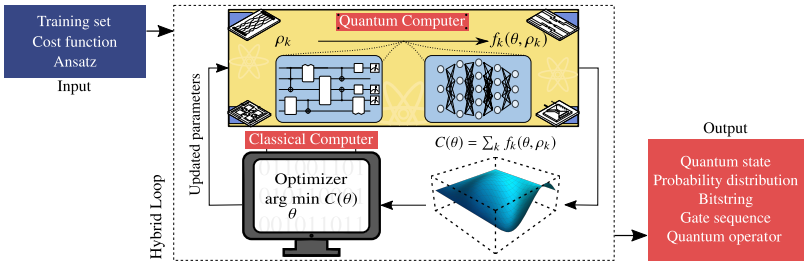
\includegraphics[width=\linewidth]{Appendices/vqadiagram.png}
    \caption{
        An illustrative diagram of VQA.
        The algorithm is a hybrid loop that receives:
        A cost function $C(\theta)$ for $\theta$ is a set of parameters that encodes the solution;
        An ansatz that receives trainable parameter $\theta$ to solve the task;
        A set of training data $\{\rho_k\}$.
        We use the quantum computer to calculate the cost for each iteration, then use an optimisation algorithm in a classical computer to find the global minima in the cost landscape $C(\theta)$ and thus satisfy the problem in Eq. (\ref{Eqn: optimize theta with ansatz}).
        VQA's result is an approximation of the problem solution, which can take forms as in the red box.
        Figure from Cerezo et al. \cite{cerezo2021variational}.
    }
    \label{Fig: VQA diagram}
\end{figure}







